\documentclass[11pt]{article}
\usepackage[margin=0.92in]{geometry}
\usepackage{amsmath,amssymb,amsthm,graphicx,microtype}
\usepackage[hidelinks]{hyperref}

\newtheorem{theorem}{Theorem}
\newcommand{\Torus}{\mathbb T}
\newcommand{\Prob}{\mathcal P}
\newcommand{\Leb}{\mathrm{Leb}}
\newcommand{\wstar}{w^*}
\setlength{\parindent}{0pt}
\setlength{\parskip}{0.6em}

\title{Fixed Dynamics Disprove Two Ces\`aro-Residuality Questions}
\author{Run \texttt{fa\_banach\_001}, lane 3}
\date{22 July 2026}

\begin{document}
\maketitle

\textbf{Status.} Candidate counterexamples, likely valid, to Questions 5.6
and 5.9 as stated in Badea--Grivaux \cite{BadeaGrivaux}. These are
literal-formulation counterexamples: they do not answer the narrower and
substantive case in which the acting dynamics are required to be independent
of the invariance dynamics.

\section{Source questions}

For an integer $m\geq 1$, let $T_m$ be the pushforward on probability
measures induced by $x\mapsto mx\pmod 1$ on $\Torus$. Let
$\Prob_p(\Torus)$ be the compact space of $T_p$-invariant probability
measures, and let $\Prob_{p,c}(\Torus)$ denote its nonatomic members.
Section 5.b of \cite{BadeaGrivaux} defines
\[
 G''_{p,(c_n)}
 =
 \left\{
 \mu\in\Prob_{p,c}(\Torus):
 \frac1N\sum_{n=0}^{N-1}T_{c_n}\mu
 \xrightarrow{\wstar}\Leb
 \right\}.
\]
Question 5.6 asks whether this set is residual in
$\Prob_p(\Torus)$ for every $p\geq2$ and every strictly increasing
integer sequence $(c_n)_{n\geq0}$.

In dimension $d\geq2$, for nonsingular integer matrices $A,B$, the paper
similarly defines
\[
 G''_{A,B}
 =
 \left\{
 \mu\in\Prob_{A,c}(\Torus^d):
 \frac1N\sum_{n=0}^{N-1}T_{B^n}\mu
 \xrightarrow{\wstar}\Leb_d
 \right\}.
\]
Question 5.9 asks whether $G''_{A,B}$ is residual in
$\Prob_A(\Torus^d)$ for every such pair $A,B$.
The exact statements occur on article pages 28--29:

\begin{center}
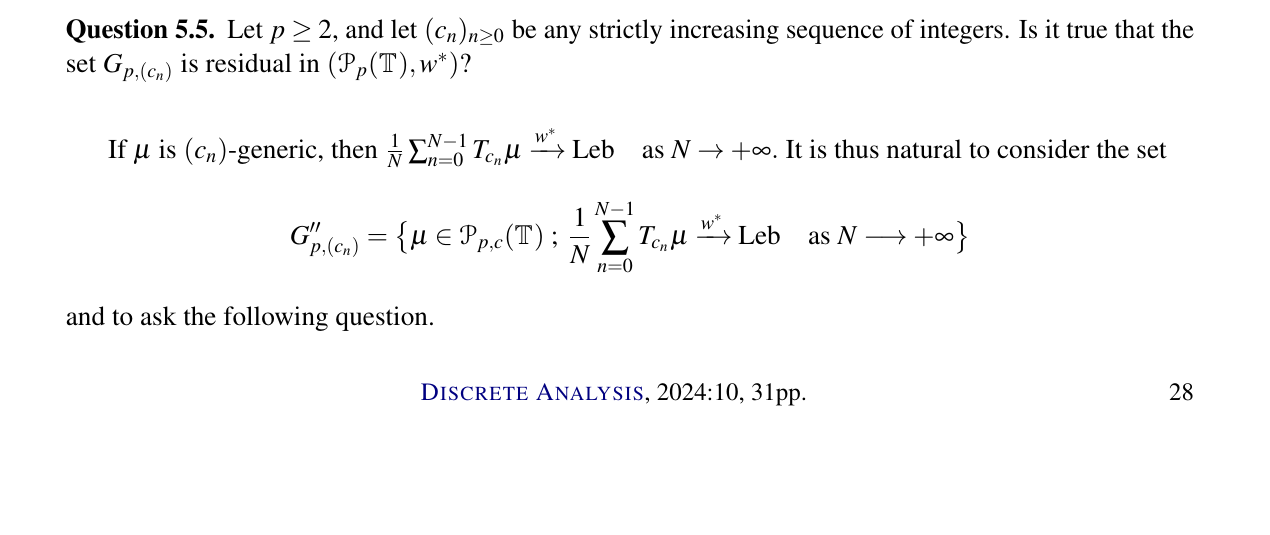
\includegraphics[width=\textwidth]{figures/question_5_6_definition_crop.png}
\end{center}

\begin{center}
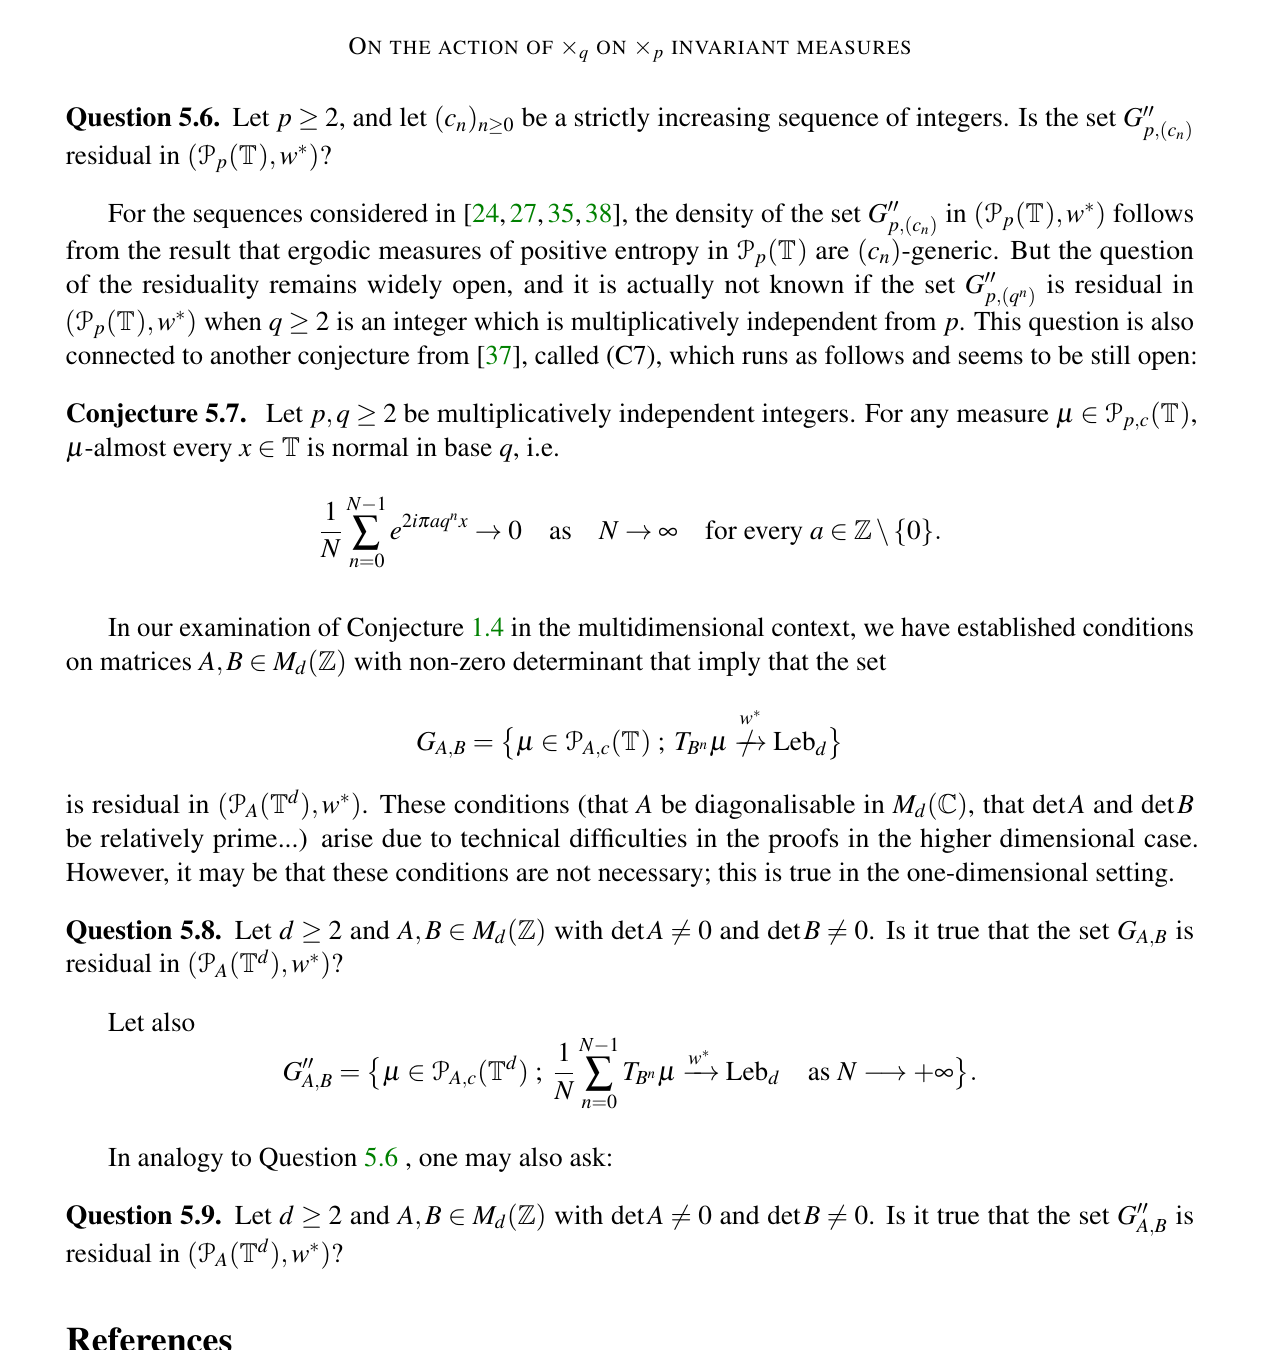
\includegraphics[width=\textwidth]{figures/questions_5_6_5_9_crop.png}
\end{center}

\section{Proof Intuition}

Both questions quantify over dynamics that are allowed to coincide with the
dynamics defining invariance. If $\mu$ is $T_p$-invariant and
$c_n=p^n$, then every term $T_{c_n}\mu$ equals $\mu$. The Ces\`aro
averages therefore cannot wash $\mu$ out to Lebesgue measure: they are the
constant sequence $\mu$. Hence the proposed generic set is only the
Lebesgue measure itself. The same fixed-point obstruction works in higher
dimension by choosing $B=A$; the concrete choice $A=B=2I_d$ already suffices.

\section{Counterexamples}

\begin{theorem}\label{thm:main}
The answers to Questions 5.6 and 5.9 of \cite{BadeaGrivaux}, as stated, are
both negative.

More precisely:
\begin{enumerate}
\item For every $p\geq2$, if $c_n=p^n$, then
      $G''_{p,(c_n)}=\{\Leb\}$, which is not residual in
      $\Prob_p(\Torus)$.
\item For every $d\geq2$, if $A=B=2I_d$, then
      $G''_{A,B}=\{\Leb_d\}$, which is not residual in
      $\Prob_A(\Torus^d)$.
\end{enumerate}
\end{theorem}

\begin{proof}
Pushforwards under multiplication obey $T_aT_b=T_{ab}$. Fix $p\geq2$
and put $c_n=p^n$. This is a strictly increasing sequence of integers.
If $\mu\in\Prob_p(\Torus)$, then $T_p\mu=\mu$, and induction gives
\[
 T_{c_n}\mu=T_{p^n}\mu=T_p^n\mu=\mu
 \qquad(n\geq0).
\]
Consequently, for every $N\geq1$,
\[
 \frac1N\sum_{n=0}^{N-1}T_{c_n}\mu=\mu.
\]
For a nonatomic $\mu$, these averages converge weak-star to $\Leb$ if
and only if $\mu=\Leb$. Thus
$G''_{p,(p^n)}=\{\Leb\}$.

The weak-star space $\Prob_p(\Torus)$ is Hausdorff and contains the
distinct point mass $\delta_0$, since $T_p\delta_0=\delta_0$.
Therefore the singleton $\{\Leb\}$ is not dense. A residual subset, in
the convention of the source paper, must contain a dense $G_\delta$ set,
so $G''_{p,(p^n)}$ is not residual. This disproves Question 5.6.

Now fix $d\geq2$ and take $A=B=2I_d$. Both matrices are integral and
have determinant $2^d\neq0$, so they meet all hypotheses of Question 5.9.
For every $\mu\in\Prob_A(\Torus^d)$,
\[
 T_{B^n}\mu=T_{A^n}\mu=T_A^n\mu=\mu.
\]
The same averaging identity shows that
$G''_{A,B}=\{\Leb_d\}$. But $\Prob_A(\Torus^d)$ also contains the
distinct invariant point mass $\delta_0$, so this singleton is not dense
and hence is not residual. This disproves Question 5.9.
\end{proof}

\section{Verification and scope}

Every hypothesis is visible in the construction. The sequence
$(p^n)_{n\geq0}$ is strictly increasing; $2I_d$ is a nonsingular integer
matrix; $\Leb$ and $\Leb_d$ are nonatomic and invariant; and $\delta_0$
provides an explicit second point in each ambient invariant-measure space.
No external theorem beyond the definitions is used.

The paper immediately singles out the case $c_n=q^n$ with $q$
multiplicatively independent from $p$ as widely open. Our example has
$q=p$ and therefore does not settle that intended independence regime.
Likewise, it does not address a multidimensional variant imposing a genuine
independence or coprimality condition between $A$ and $B$. Questions 5.5
and 5.8, which concern failure of pointwise weak-star convergence rather
than convergence of Ces\`aro averages, are not contradicted.

\section{Novelty check}

The run indexes were searched for arXiv:2303.01089, the paper title,
Questions 5.6 and 5.9, Ces\`aro residuality, and the fixed sequences
$c_n=p^n$ and $B=A$. No prior packet or attempt was found. Bounded web
searches on 22 July 2026 used the exact question numbers with the arXiv id,
the authors' names with the displayed $G''$ notation, and the phrases
\texttt{c\_n = p\^n}, \texttt{T\_p-invariant}, and
\texttt{Cesaro residual}. They found the source paper and its journal
page but no later answer or discussion of this obstruction. Novelty
confidence is moderate: the proof is elementary and may be an unrecorded
formulation correction.

\section{Human-review recommendation}

Review as a likely valid literal counterexample to both universal questions.
The decisive checks are that the published Questions 5.6 and 5.9 impose no
independence condition, and that residuality is taken in the full spaces
$\Prob_p(\Torus)$ and $\Prob_A(\Torus^d)$, respectively.

\begin{thebibliography}{1}
\bibitem{BadeaGrivaux}
C.~Badea and S.~Grivaux,
\emph{Around Furstenberg's times $p$, times $q$ conjecture: times
$p$-invariant measures with some large Fourier coefficients},
Discrete Analysis 2024:10 (2024), 31 pp.,
doi:\href{https://doi.org/10.19086/da.124611}{10.19086/da.124611};
arXiv:\href{https://arxiv.org/abs/2303.01089}{2303.01089}.
\end{thebibliography}

\end{document}

